\documentclass[submit]{harvardml}

\course{CS181-S22}
\assignment{Assignment \#4}
\duedate{11:59pm EST, March 25, 2022} 

\usepackage[OT1]{fontenc}
\usepackage[colorlinks,citecolor=blue,urlcolor=blue]{hyperref}
\usepackage[pdftex]{graphicx}
\usepackage{graphicx}
\usepackage{caption}
\usepackage{fullpage}
\usepackage{soul}
\usepackage{amsmath}
\usepackage{framed}
\usepackage{amssymb}
\usepackage{color}
\usepackage{todonotes}
\usepackage{listings}
\usepackage{common}

\usepackage[mmddyyyy,hhmmss]{datetime}

\usepackage{comment}
\usepackage{subcaption}
\usepackage{mdframed}

\definecolor{verbgray}{gray}{0.9}

\lstnewenvironment{csv}{
  \lstset{backgroundcolor=\color{verbgray},
  frame=single,
  framerule=0pt,
  basicstyle=\ttfamily,
  columns=fullflexible}}{}
 
\begin{document}

\begin{center}
{\Large Homework 4: SVM, Clustering, and Ethics}\\
\end{center}

\subsection*{Introduction}

This homework assignment will have you work with SVMs, 
clustering, and engage with the ethics lecture.  We encourage you to
read Chapters 5 and 6 of the course textbook.

Please submit the \textbf{writeup PDF to the Gradescope assignment `HW4'}. Remember to assign pages for each question.

Please submit your \textbf{\LaTeX\ file and code files to the Gradescope assignment `HW4 - Supplemental'}. 

\newpage

%%%%%%%%%%%%%%%%%%%%%%%%%%%%%%%%%%%%%%%%%%%%%
% Problem 1
%%%%%%%%%%%%%%%%%%%%%%%%%%%%%%%%%%%%%%%%%%%%%
\begin{problem}[Fitting an SVM by hand, 10pts]

  For this problem you will solve an SVM by hand, relying on principled rules and SVM properties. 
  For making plots, however, you are allowed to use a computer or other graphical tools.

Consider a dataset with the following 7 data points each with $x \in \reals$ and $y \in \{ -1, +1 \}$ : \[\{(x_i, y_i)\}_{i = 1}^7 =\{(-3 , +1) , (-2 , +1 ) , (-1,  -1 ), (0, +1), ( 1 , -1 ), ( 2 , +1 ) , (3 , +1 )\}\] Consider
mapping these points to $2$ dimensions using the feature vector $\bphi(x) =  (x, -\frac{8}{3}x^2 + \frac{2}{3}x^4 )$. The hard margin classifier training problem is:
%
\begin{align*}
  &\min_{\mathbf{w}, w_0} \frac{1}{2}\|\mathbf{w}\|_2^2 \label{eq:dcp} \\
  \quad \text{s.t.} \quad & y_i(\mathbf{w}^\top \bphi(x_i) + w_0) \geq 1,~\forall i \in \{1,\ldots, n\}\notag
\end{align*}

Make sure to follow the logical structure of
the questions below when composing your answers, and to justify each step.

\begin{enumerate}
\item Plot the transformed training data in $\reals^2$ and draw the
  optimal decision boundary of the max margin classifier. You can
  determine this by inspection (i.e. by hand, without actually doing
  any calculations).

\item What is the value of the margin achieved by the optimal decision
  boundary found in Part 1?

\item Identify a unit vector that is orthogonal to the decision boundary.

\item Considering the discriminant
  $h(\bphi(x);\boldw,w_0)=\boldw^\top\bphi(x) +w_0$, give an
  expression for {\em all possible} $(\boldw,w_0)$ that define the
  optimal decision boundary from 1.1.  Justify your answer.

  Hint: The boundary is where the discriminant is equal to 0.  Use
  what you know from 1.1 and 1.3 to solve for $\boldw$ in terms of
  $w_0$.  (If you solve this problem in this way, then $w_0$
  corresponds to your free parameter to describe the set of all
  possible $(\boldw,w_0)$.)
  
\item Consider now the training problem for this dataset. Using your
  answers so far, what particular solution to $\boldw$ will be optimal
  for the optimization problem?

\item What is the corresponding optimal value of $w_0$ for the
  $\boldw$ found in Part 5 (use your result from Part 4 as guidance)?
  Substitute in these optimal values and write out the discriminant
  function $h(\bphi(x);\boldw,w_0)$ in terms of the variable $x$ .


\item Which points could possibly be support vectors of the classifier?  Confirm that
  your solution in Part 6 makes the constraints above tight---that is,
  met with equality---for these candidate points.

\item Suppose that we had decided to use a different feature mapping
    $\bphi'(x) = (x, -\frac{31}{12}x^2 + \frac{7}{12}x^4 )$.  Does
    this feature mapping still admit a separable solution?  How does
    its margin compare to the margin in the previous parts?  Based on
    this, which set of features might you prefer and why? 
    
\end{enumerate}

\end{problem}

\subsection*{Solution}

\begin{enumerate}
	\item By inspection, the optimal decision boundary of the max margin classifier is the line where the second dimension is equal to -1.
	
	\begin{center}
		\includegraphics[width=0.7\textwidth]{SVM}
	\end{center}
	
	\item The value of the margin is 1, since the datapoints with $-2 \leq x_i \leq 2$ are all distance 1 from the optimal decision boundary.
	
	\item The unit vector
	%$\begin{bmatrix} 0 \\ 1 \end{bmatrix}$
	$(0, 1)^\top$
	is orthogonal to the decision boundary.
	
	\item The decision boundary is the line where the discriminant is equal to 0, which occurs here when $\phi_2(x) = -1$. Plugging this in to the discriminant equation,
	\begin{align*}
		0 &= h(\bphi(x);\boldw,w_0) \\
		&= \boldw^\top\bphi(x) +w_0 \\
		&= w_1\phi_1(x) + w_2\phi_2(x) + w_0 \\
		&= w_1\phi_1(x) - w_2 + w_0.
	\end{align*}
	Since $\boldw$ is orthogonal to the decision boundary and thus parallel to $(0, 1)^\top$, we have $w_1 = 0$, leaving
	$$w_2 = w_0.$$
	Therefore, the set of all possible $(\boldw, w_0)$ that define the optimal decision boundary is
	$$\{(\boldw, w_0) : w_1 = 0, w_2 = w_0\}.$$

	\item The training problem is
	$$\min_{\boldw, w_0} \frac12||\boldw||_2^2 \quad \text{s.t.} \quad y_i(\boldw^\top\phi(x_i) + w_0) \geq 1, \forall i \in \{1, \ldots, n\}.$$
	From Part 4, we must have $w_1 = 0$ and $w_2 = w_0$, so the constraint equation reduces to
	$$y_i(w_2\phi(x_i) + w_2) \geq 1$$
	$$y_iw_2(\phi(x_i) + 1) \geq 1.$$
	Examining the training set, the minimal $w_2$ that satisfies this constraint for all training points is $w_2 = 1$, giving
	$$\boldw = (0, 1)^\top.$$
	%We could also have seen this by recalling that $\boldw$ is parallel to $(0, 1)^\top$, the margin is 1, and that in the training problem we set our constraints to make the margin equal to $\frac{1}{||w||_2}$.
	
	\item From Part 4, the corresponding optimal value of $w_0$ is simply
	$$w_0 = w_2 = 1.$$
	This makes the discriminant function
	\begin{align*}
		h(\bphi(x);\boldw,w_0) &= \phi_2(x) + 1 \\
		&= -\frac{8}{3}x^2 + \frac{2}{3}x^4 + 1.
	\end{align*}

	\item Only the points $i \in \{2, 3, 4, 5, 6\}$, which have $x_i \in \{-2, -1, 0, 1, 2\}$, could possibly be support vectors of the classifier, since if either of the points $i \in \{-3, 3\}$ were on the margin boundary, some of the training points would have to be misclassified. The constraints for the possible support vector points are
	\begin{align*}
		&y_2(h(\phi(-2); \boldw, w_0)) = 1(0 + 1) &= 1 \\
		&y_3(h(\phi(-1); \boldw, w_0)) = -1(-2 + 1) &= 1 \\
		&y_4(h(\phi(0); \boldw, w_0)) = 1(0 + 1) &= 1 \\
		&y_5(h(\phi(1); \boldw, w_0)) = -1(-2 + 1) &= 1 \\
		&y_6(h(\phi(2); \boldw, w_0)) = 1(0 + 1) &= 1
	\end{align*}
	
	\item The alternate feature mapping plot is:
	\begin{center}
	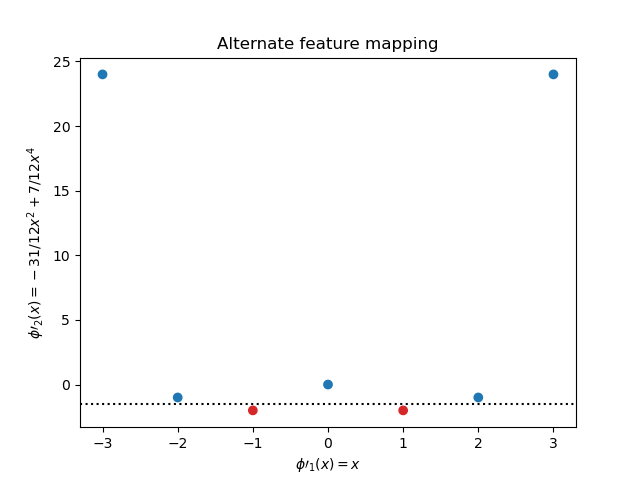
\includegraphics[width=0.7\textwidth]{svm_alt}
	\end{center}
	This still admits a separable solution, since there is space for a line between the classes, including an optimal line where the second dimension is equal to -1.5. The margin, however, is only 0.5, which is smaller than in the original feature mapping. Based on this, I would prefer the original set of features $\phi$, because they allow for a larger margin and therefore a greater degree of separation between the classes, ideally making the boundary more robust to future data.
\end{enumerate}


%%%%%%%%%%%%%%%%%%%%%%%%%%%%%%%%%%%%%%%%%%%%%
% Problem 2
%%%%%%%%%%%%%%%%%%%%%%%%%%%%%%%%%%%%%%%%%%%%%

\begin{problem}[K-Means and HAC, 20pts]

For this problem you will implement K-Means and HAC from scratch to cluster image data. You may use \texttt{numpy} but no third-party ML implementations (eg. \texttt{scikit-learn}).

We've provided you with a subset of the MNIST dataset, a collection of
handwritten digits used as a benchmark for image recognition (learn more at
\url{http://yann.lecun.com/exdb/mnist/}). MNIST is widely used in supervised learning, and modern algorithms do very well. 

You have been given
representations of MNIST images, each of which is a $784\times1$
greyscale handwritten digit from 0-9. Your job is to implement K-means and HAC on MNIST, and to test whether these relatively
simple algorithms can cluster similar-looking images together.

The code in \texttt{T4\_P2.py} loads the images into your environment into two arrays -- \texttt{large\_dataset}, a 5000x784 array, will be used for K-means, while \texttt{small\_dataset}, a 300x784 array, will be used for HAC. In your code, you should use the $\ell_2$ norm (i.e. Euclidean distance) as your distance metric.

\textbf{Important:} Remember to include all of your plots in your PDF submission!

\textbf{Checking your algorithms:} Instead of an Autograder file, we have provided a similar dataset, \texttt{P2\_Autograder\_Data}, and some visualizations, \texttt{HAC\_visual} and \texttt{KMeans\_visual}, for how K-means and HAC perform on this data. Run your K-means (with $K=10$ and \texttt{np.random.seed(2)}) and HAC on this second dataset to confirm your answers against the provided visualizations. Do \textbf{not} submit the outputs generated from \texttt{P2\_Autograder\_Data}. Load this data with \texttt{data = np.load(`P2\_Autograder\_Data.npy')}.

\begin{enumerate}

\item Starting at a random initialization and $K = 10$, plot the
  K-means objective function (the residual sum of squares) as a
  function of iterations and verify that it never increases.

\item For $K=10$ and for 3 random restarts, print the mean image (aka
  the centroid) for each cluster. There should be 30 total images. Code 
  that creates plots for parts 2, 3, and 4 can be found in \texttt{T4\_P2.py}.

\item Repeat Part 2, but before running K-means, standardize or center
  the data such that each pixel has mean 0 and variance 1 (for any
  pixels with zero variance, simply divide by 1). For $K=10$ and 3
  random restarts, show the mean image (centroid) for each
  cluster. Again, present the 30 total images in a single
  plot. Compare to Part 2: How do the centroids visually differ? Why?

\item Implement HAC for min, max, and centroid-based linkages. Fit
  these models to the \texttt{small\_dataset}.  For each of these 3
  linkage criteria, find the mean image for each cluster when using
  $10$ clusters. Display these images (30 total) on a single plot.

  How do the ``crispness'' of the cluster means and the digits
  represented compare to mean images for k-means?  
  Why do we only ask you to run HAC once?  

  \textbf{Important Note:} For this part ONLY, you may use
  \texttt{scipy}'s \texttt{cdist} function to calculate Euclidean
  distances between every pair of points in two arrays.

\item For each of the HAC linkages, as well as one of the runs of your
  k-means, make a plot of ``Number of images in cluster" (y-axis)
  v. ``Cluster index" (x-axis) reflecting the assignments during the
  phase of the algorithm when there were $K=10$ clusters.

  Intuitively, what do these plots tell you about the difference
  between the clusters produced by the max and min linkage criteria?

  Going back to the previous part: How does this help explain the
  crispness and blurriness of some of the clusters?  
\end{enumerate}
\end{problem}

\newpage
\begin{framed}
\noindent\textbf{Problem 2} (cont.)\\
\begin{enumerate}
\setcounter{enumi}{5}
\item For your K-means with $K = 10$ model and HAC min/max/centroid
  models using $10$ clusters on the \texttt{small\_dataset} images,
  use the \texttt{seaborn} module's \texttt{heatmap} function to plot
  a confusion matrix between each pair of clustering methods.  This
  will produce 6 matrices, one per pair of methods. The cell at the
  $i$th row, $j$th column of your confusion matrix is the number of
  times that an image with the cluster label $j$ of one method has
  cluster $i$ in the second method.  Which HAC is closest to k-means?
  Why might that be?

\item Suppose instead of comparing the different clustering methods to
  each other, we had decided to compute confusions of each clustering
  method to the \emph{true} digit labels (you do \emph{not} have to
  actually compute this).  Do you think how well the clustering match
  the true digits is reasonable evaluation metric for the clustering?
  Explain why or why not.
  
\end{enumerate}
\end{framed}


\subsection*{Solution}

\begin{enumerate}
	\item The objective function never increases:
		
	\begin{center}
		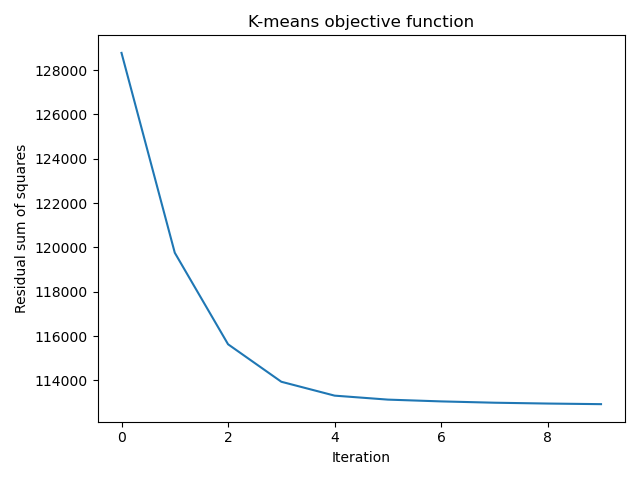
\includegraphics[width=0.7\textwidth]{kmeans_obj}
	\end{center}

	\item The mean images are:

	\begin{center}
		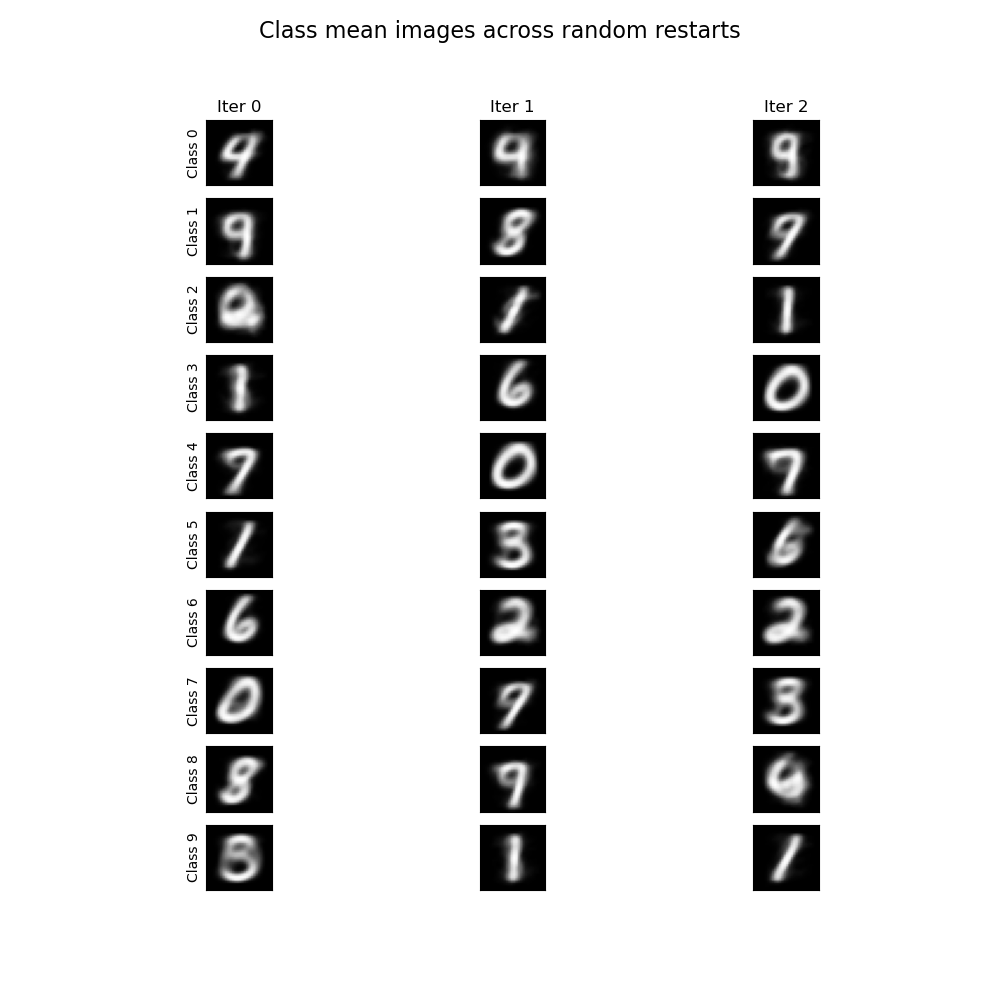
\includegraphics[width=0.7\textwidth]{kmeans}
	\end{center}

	\item The mean images, using standardized data, are:

	\begin{center}
		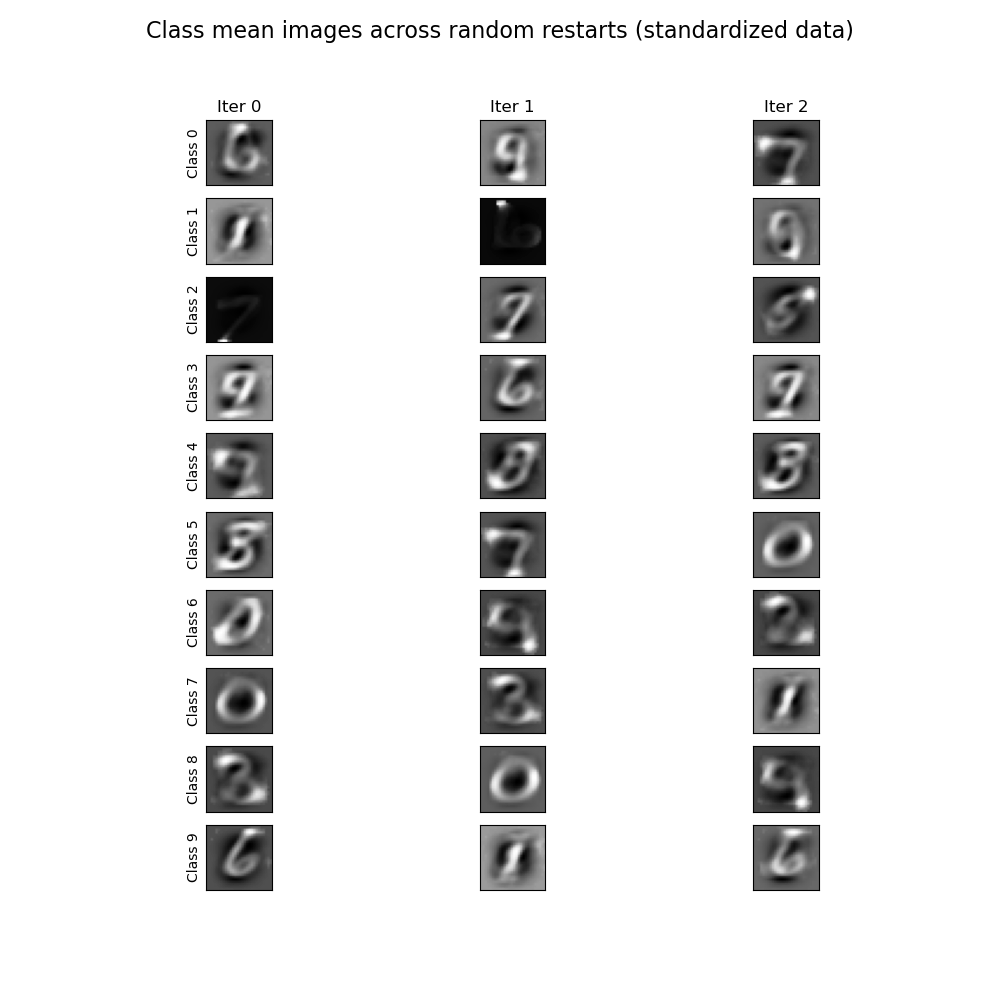
\includegraphics[width=0.7\textwidth]{kmeans_standardized}
	\end{center}
	
	The most obvious visual difference in comparison to the non-standardized data from Part 2 is that the outer regions of the images that were previously black are now grey, since with standardized data these regions have mean values around zero. In contrast, regions with higher variance, where some source images are white and others black, are the most extreme parts of the mean images visually. In terms of the accuracy of the actual classes generated by K-Means, the standardized data seems to be comparable to the non-standardized data, with both data sets resulting in some clear classes for digits like 0, 1, and 6, and more muddled classes for other digits.

	\item The HAC mean images are:
	
	\begin{center}
		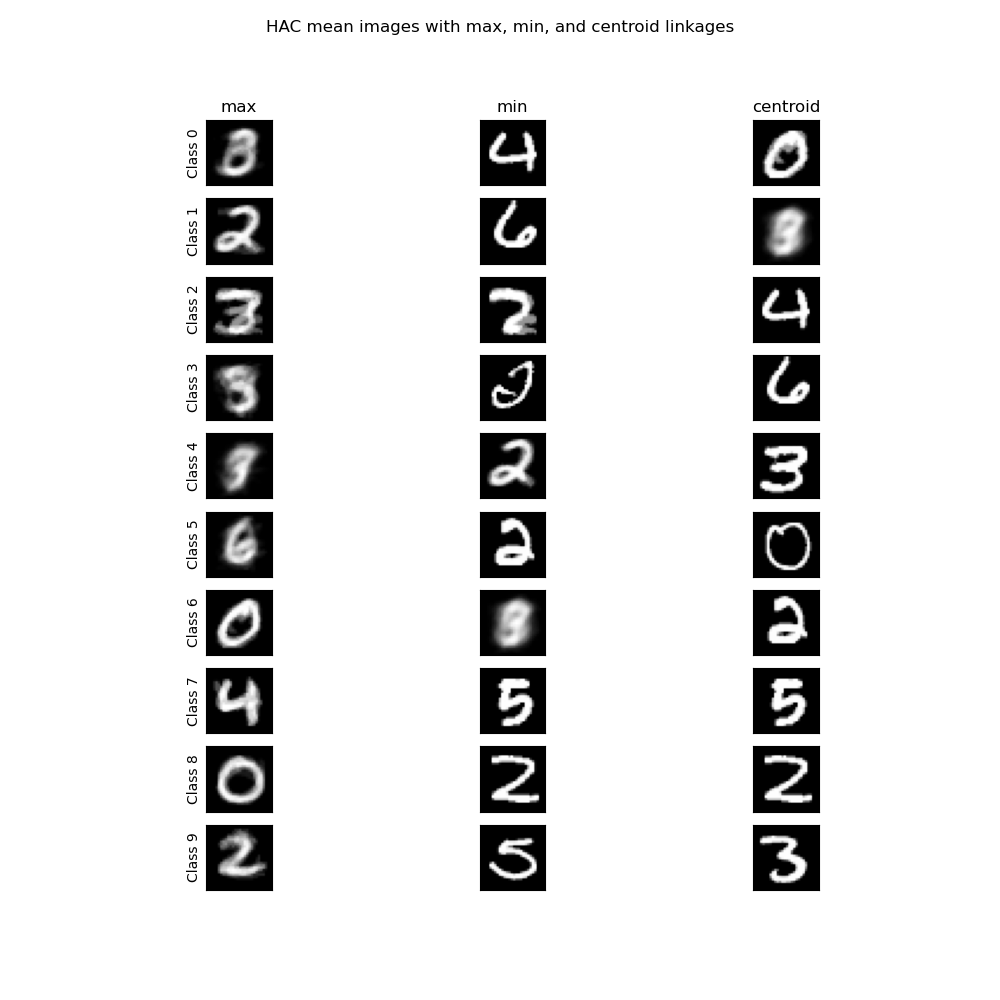
\includegraphics[width=0.7\textwidth]{HAC}
	\end{center}
	The cluster means for max-linkage are slightly blurrier than those for K-Means, but for min- and centroid-linkage are generally much crisper than those for K-Means. However, one of the mean images for each of the min- and centroid-linkage types is quite blurry.

	We only need to run HAC once since, after selecting a linkage criterion, it is a deterministic algorithm, meaning the clusters would be the same in every iteration.

	\item See Figure \ref{fig:2.5}.
	
	\begin{figure}[h]
		\centering
		\begin{subfigure}[b]{0.475\textwidth}
			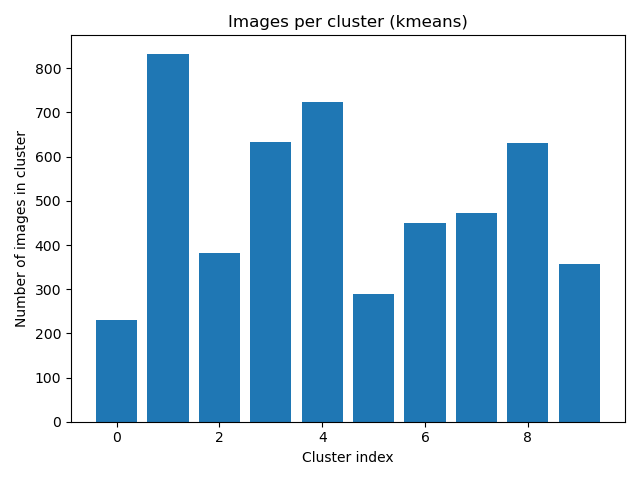
\includegraphics[width=\textwidth]{kmeans_nimages_per_cluster}
		\end{subfigure}
		\hfill
		\begin{subfigure}[b]{0.475\textwidth}
			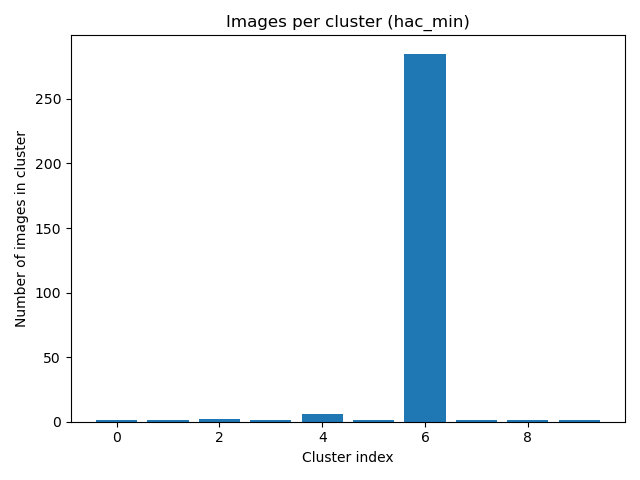
\includegraphics[width=\textwidth]{hac_min_nimages_per_cluster}
		\end{subfigure}
		\hfill
		\vskip\baselineskip
		\begin{subfigure}[b]{0.475\textwidth}
			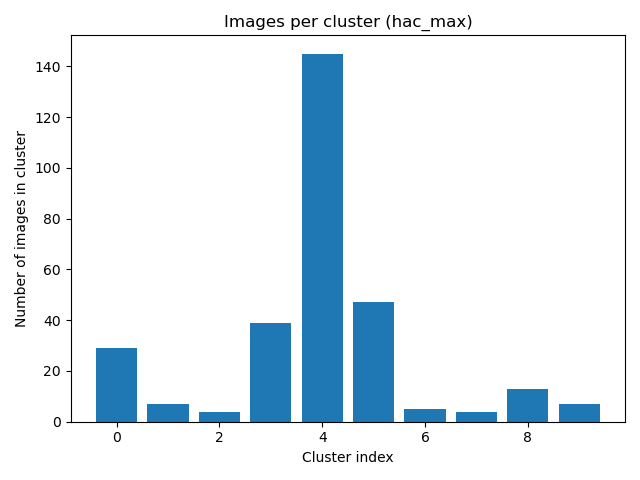
\includegraphics[width=\textwidth]{hac_max_nimages_per_cluster}
		\end{subfigure}
		\hfill
		\begin{subfigure}[b]{0.475\textwidth}
			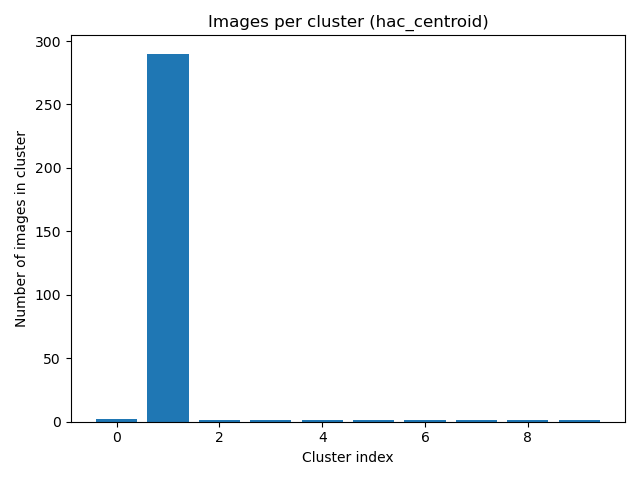
\includegraphics[width=\textwidth]{hac_centroid_nimages_per_cluster}
		\end{subfigure}
		\caption{Number of images per cluster}
		\label{fig:2.5}
	\end{figure}

	Intuitively, the plots show that the max-linkage criterion produced a variety of clusters of unequal, but still considerable, sizes. By contrast, the min-linkage criterion produced one cluster containing almost all of the images, with the rest of the clusters being much smaller. Presumably the small clusters contain those images which are farthest away from any other image.
	
	Going back to the previous part, this explains why many of the mean images in the min- and centroid-linkage models were very crisp, while one image was quite blurry. The crisp images are because many of the classes in these models contain only one or a few images, all of which are quite similar to each other, giving them a very crisp mean. By contrast, the class with most of the images has a very blurry mean, since it is comprised of images of many different digits. In a less extreme sense, the same logic helps explain why some of the max-linkage model mean images are crisper than others.
	
	\item See Figure \ref{fig:2.6}.
	
	\begin{figure}[h]
		\centering
		\begin{subfigure}[b]{0.475\textwidth}
			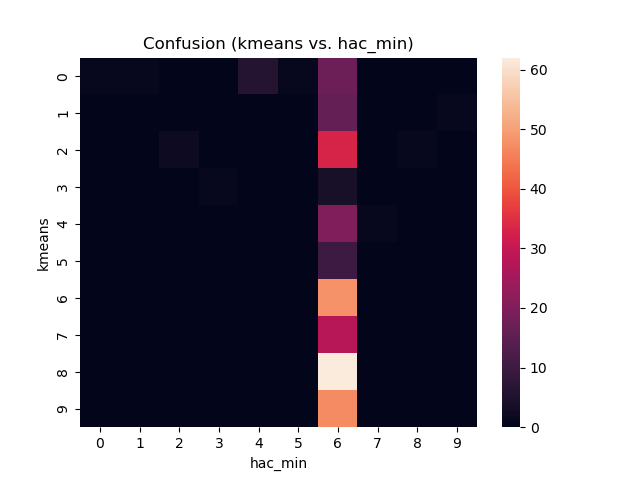
\includegraphics[width=\textwidth]{kmeans_hac_min_confusion}
		\end{subfigure}
		\hfill
		\begin{subfigure}[b]{0.475\textwidth}
			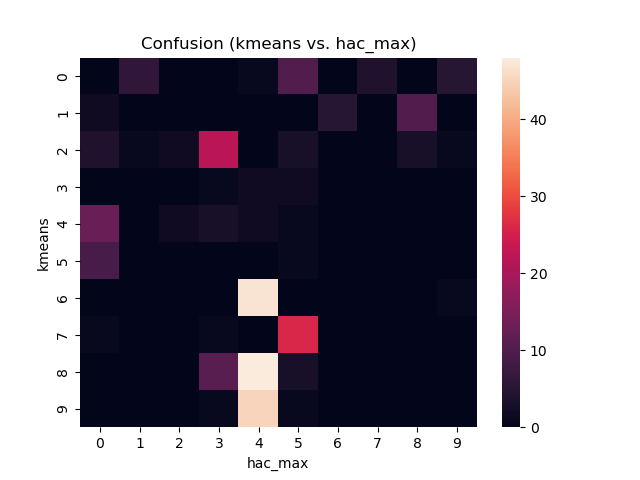
\includegraphics[width=\textwidth]{kmeans_hac_max_confusion}
		\end{subfigure}
		\hfill
		\vskip\baselineskip
		\begin{subfigure}[b]{0.475\textwidth}
			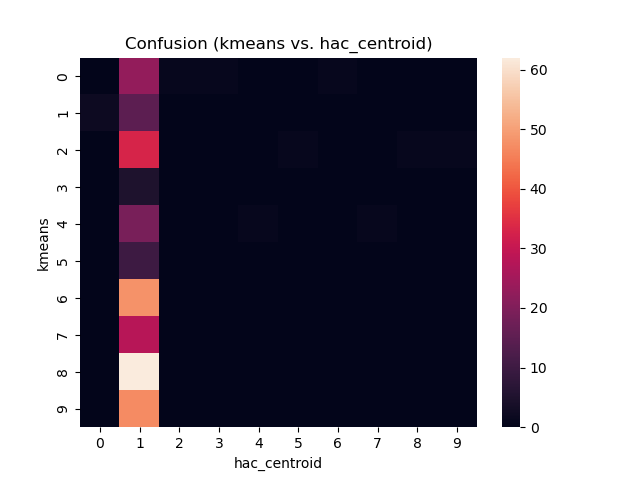
\includegraphics[width=\textwidth]{kmeans_hac_centroid_confusion}
		\end{subfigure}
		\hfill
		\begin{subfigure}[b]{0.475\textwidth}
			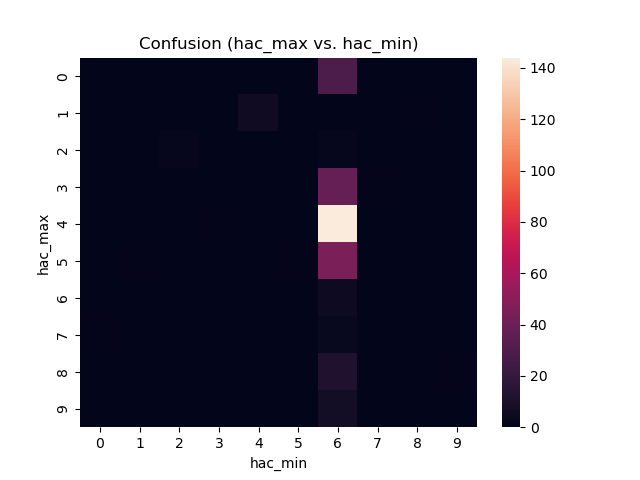
\includegraphics[width=\textwidth]{hac_max_hac_min_confusion}
		\end{subfigure}
		\hfill
		\vskip\baselineskip
		\begin{subfigure}[b]{0.475\textwidth}
			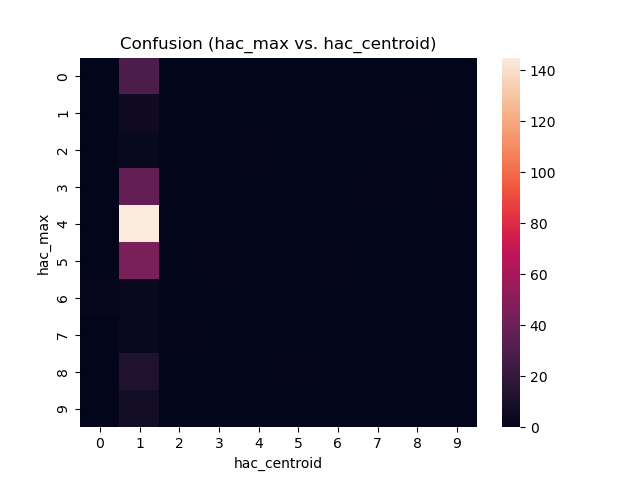
\includegraphics[width=\textwidth]{hac_max_hac_centroid_confusion}
		\end{subfigure}
		\hfill
		\begin{subfigure}[b]{0.475\textwidth}
			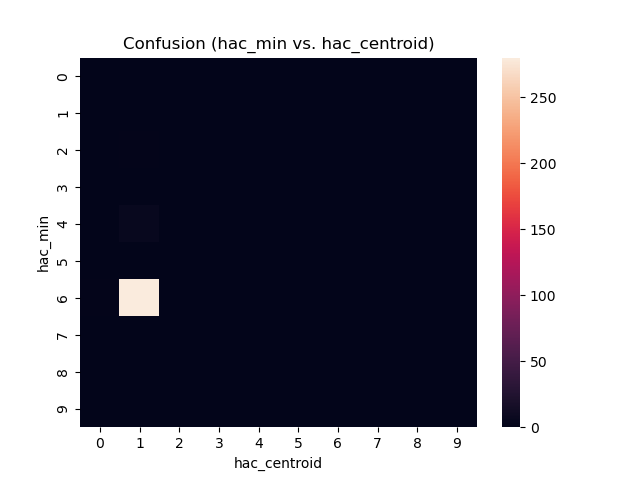
\includegraphics[width=\textwidth]{hac_min_hac_centroid_confusion}
		\end{subfigure}
		\caption{Confusion matrices}
		\label{fig:2.6}
	\end{figure}

	Max-linkage HAC is the closest to K-Means, which we can see from the non-negligible number of shared images for each class. By contrast, the min- and centroid-linkage HAC models have large vertical bars on their heatmaps which indicate that almost all of their images are in the same class, regardless of the class K-Means puts them in.
	
	Max-linkage HAC is closest to K-Means because K-Means tends to group the data points into clusters that are hypersphere-like in order to minimize the distances of points to their means. Similarly, the HAC max-linkage criterion tends to group the data points into hypersphere-like clusters in order to minimize the distance of new points to the farthest-away point in the sphere. By contrast, the min- and centroid-linkage critera can produce stringer clusters, or in this case can group most of the data points into one cluster when they are relatively evenly spread out in space, because they can start with one cluster and gradually expand it across the space to include most of the data points without incurring a substantial penalty for having a large, spread-out cluster.
	
	\item Yes, it does seem like comparing the clusterings to the true digit labels is a reasonable evaluation metric since our goal from the outset was to find a clustering method that could correctly classify the images into digits as well as possible. Comparing against the true digit labels would give us an empirical measure of how well each clustering method identifies the true clusters of images into digits.
	
\end{enumerate}

\newpage
%%%%%%%%%%%%%%%%%%%%%%%%%%%%%%%%%%%%%%%%%%%%%
% Problem 3
%%%%%%%%%%%%%%%%%%%%%%%%%%%%%%%%%%%%%%%%%%%%%

\begin{problem}[Ethics Assignment, 5pts]

Select a real-life outcome in Artificial Intelligence or Machine Learning 
that you believe is morally wrong. You can select your own outcome from 
the news or select one of the outcomes in the options below:

\begin{itemize}
    \item COMPAS, a case management tool predicting recidivism that 
        flagged “blacks are almost twice as likely as whites to be 
        labeled a higher risk but not actually re-offend” (Angwin 
        2016).
        
    \item An NLP algorithm filled in the inference “Man is to 
        \_\_\_\_ as woman is to \_\_\_\_” with “Man is 
        to computer programmer as woman is to homemaker” (Bolukbasi 
        et al, 2016).
        
    \item \url{http://www.survivalofthebestfit.com/game}: a game that 
        exemplifies algorithmic bias in resume screening
        
    \item IBM Diversity in faces: insufficient training data for 
        darker-skinned faces
        
    \item Other Unfair Algorithms: Algorithms of Oppression (a really 
        good book with tons of examples), VI-SPDAT, Allegheny Family 
        Screening Tool
        
\end{itemize}
Draw a causal chain that resulted in this outcome and circle the choice points that were the largest contributors to the outcome. At each morally relevant choice point, write two alternative decisions that could have prevented the outcome.

\end{problem}

\subsection*{Solution}

Outcome: An NLP algorithm filled in the inference “Man is to 
\_\_\_\_ as woman is to \_\_\_\_” with “Man is 
to computer programmer as woman is to homemaker” (Bolukbasi 
et al, 2016).

We present the causal chain as a list in chronological order. The choice point that is the largest contributor to the outcome is underlined. Morally relevant choice points are followed by alternative decisions.

\begin{enumerate}
	\item Development of natural language processing algorithms for applications like speech recognition and generation.

	\item \ul{The concept of word embedding is developed. Word embeddings transform words into vectors in a high-dimensional space that relates words by similarity along various dimensions.}
	
		\begin{enumerate}
			\item Alternative 1 (Naive): Don't use word embeddings, and instead use ``one-hot" or ``bag of words" representations of text. This avoids word representations having any gender bias, because the representations of words have no relationship to their meaning. However, this denies us the important benefits of word embeddings, not only for comparing similar words, but also for ease of NLP training and the representation of large vocabularies.
			\item Alternative 2: Recognize that word embeddings have the potential to encode both actual similarities and stereotypical similarities, and proceed to develop the theory of word embeddings with this in mind.
		\end{enumerate}
	
	\item Embeddings like word2vec train on large corpora using ``second-order" techniques, which uncover both implicit meaning and implicit bias in texts, rather than ``first-order" techniques, which simply count the number of times words occur near each other. First-order techniques might not, for example, not consider the word ``nurse" feminine, since the phrase ``male nurse" occurs more often in the world than ``female nurse," because the ``female" part is often left implicit when describing a ``female nurse." Second-order techniques uncover the implicit bias and consider the word ``nurse" feminine.
		\begin{enumerate}
			\item Alternative 1 (Naive): Use only first-order techniques. However, as in the example of ``nurse," this could create bias in the other direction, where ``nurse" becomes associated with males. Additionally, first-order techniques severely limit the expressivity of the resulting embeddings.
			\item Alternative 2: Attempt to hardcode gender-neutrality into training algorithms for word embeddings, so that bias is removed in the training process.
		\end{enumerate}
	
	\item Researchers train use word2vec to train an embedding called w2vNEWS on a corpus of Google News texts consisting of 3 million English words, placing them in 300 dimensions. Even though the news articles are primarily written by professional journalists and should ideally exhibit little gender bias, bias still occurs in the embeddings.
		\begin{enumerate}
			\item Alternative 1 (Naive): Systematically review the corpus by hand for gender bias, both implicit and explicit, and edit articles to remove it. However, this could be impractically time consuming. Additionally, there are no guarantees that the human reviewers would find or successfully correct all bias due to their own biases. It would not be possible to carry this process out using ML, since the reviewing model would itself have bias if not trained on unbiased data.
			\item Alternative 2: De-bias word embeddings after training using the techniques developed by Bolukbasi et al. This is probably the best alternative of all those considered. In the future, this de-biasing process could hopefully be automatically applied to all word embeddings after they are generated to make all future embeddings free of gender- and other-biases. 
		\end{enumerate}

	\item An NLP algorithm filled in the inference “Man is to \_\_\_\_ as woman is to \_\_\_\_” with “Man is to computer programmer as woman is to homemaker”
\end{enumerate}

\newpage
%%%%%%%%%%%%%%%%%%%%%%%%%%%%%%%%%%%%%%%%%%%%%
% Name and Calibration
%%%%%%%%%%%%%%%%%%%%%%%%%%%%%%%%%%%%%%%%%%%%%
\subsection*{Name}

Alex Encalada-Stuart

\subsection*{Collaborators and Resources}
Whom did you work with, and did you use any resources beyond cs181-textbook and your notes?

No one and no

Did you attend office hours for help with this homework?

No

\subsection*{Calibration}
Approximately how long did this homework take you to complete (in hours)? 

16

\end{document}